\subsection{Experiments}

\subsubsection{Performance of our algorithm for signal reconstruction}
We perform experiments on a synthetic signal generated randomly with $n=1000$ and $s={3,6,9,12}$. We compute the initial estimate $\mathbf{x^0}$ using first order estimator method described in~\ref{sec:init}. we plot the variation of the relative reconstruction error ($\frac{\norm{\mathbf{x^*-x^N}}}{\norm{\mathbf{x^*}}}$) with number of measurements $m$ for both the variants of sparse recovery algorithm as described in~\ref{sec:altmin}.

It is important to note that unlike the absolute value function, the modulo function described in Fig.~\ref{fig:graph} is not scale-invariant. The modulo function works over the quantities $y_{c,i}=\langle \mathbf{a_i} \cdot \mathbf{x^*} \rangle, i=1,..,m$; and it is defined over the parameter $R$; thus depending on the magnitudes of $y_{c,i}$ and $R$ relative to each other, the behavior of the measurement model and the reconstruction algorithm would be altered. For instance, if the value of $R$ is too small compared to the range of the $y_{c,i}$, the modulo operation would hardly have any effect on the measurements, leaving $\mathbf{y_c \approx y}$. To analyze such variations, we fix the $R =1$ in our experiments, while varying the signal strength to vary the magnitudes of $y_{c,i}$. We measure the signal strength by the norm of the original signal ($\norm{\mathbf{{x}^*}}=1$).

Another important factor affecting the reconstruction is the quality of the initial estimate ($\mathbf{{x}^0}$) obtained through first order estimation. As described in~\ref{sec:init}, the quality of the initial estimate is a direct function of number of measurements ($m$). As we set $m$ higher, the initial estimate $\mathbf{{x}^0}$ would move closer to the original signal $\mathbf{{x}^*}$. For our experiments, we consider two ranges of $m$: $m \in [100,1000]$ and $m \in [1000,10000]$.


\begin{center}
	\begin{table}[h]
		\centering
		\begin{tabular}{ccc}\toprule
			\multicolumn{3}{c}{\small{\textbf{Fixed:} $n=1000,\norm{\mathbf{{x}^*}}=1$}} \\ \midrule
			\multicolumn{3}{c}{\textbf{Justice Pursuit}}
			\\\cmidrule(r){1-3}%\cmidrule(r){3-4}  
			\small{$R =1$}&\small{$R=2$}&\small{$R=4$} \\\midrule
			\hyperref[fig:plot-2-1]{Figure~\ref{fig:plot-2-1}} & \hyperref[fig:plot-2-2]{Figure~\ref{fig:plot-2-2}}
			& \hyperref[fig:plot-2-3]{Figure~\ref{fig:plot-2-3}} \\
			\bottomrule
		\end{tabular}
		\caption{The Results}\label{Tab3}
	\end{table} 	
\end{center}
In the Table~\ref{Tab3}, we provide experimental results for each of the combination above.

\begin{figure}[h!]
	\begin{center}
		%\vspace{-0em}
		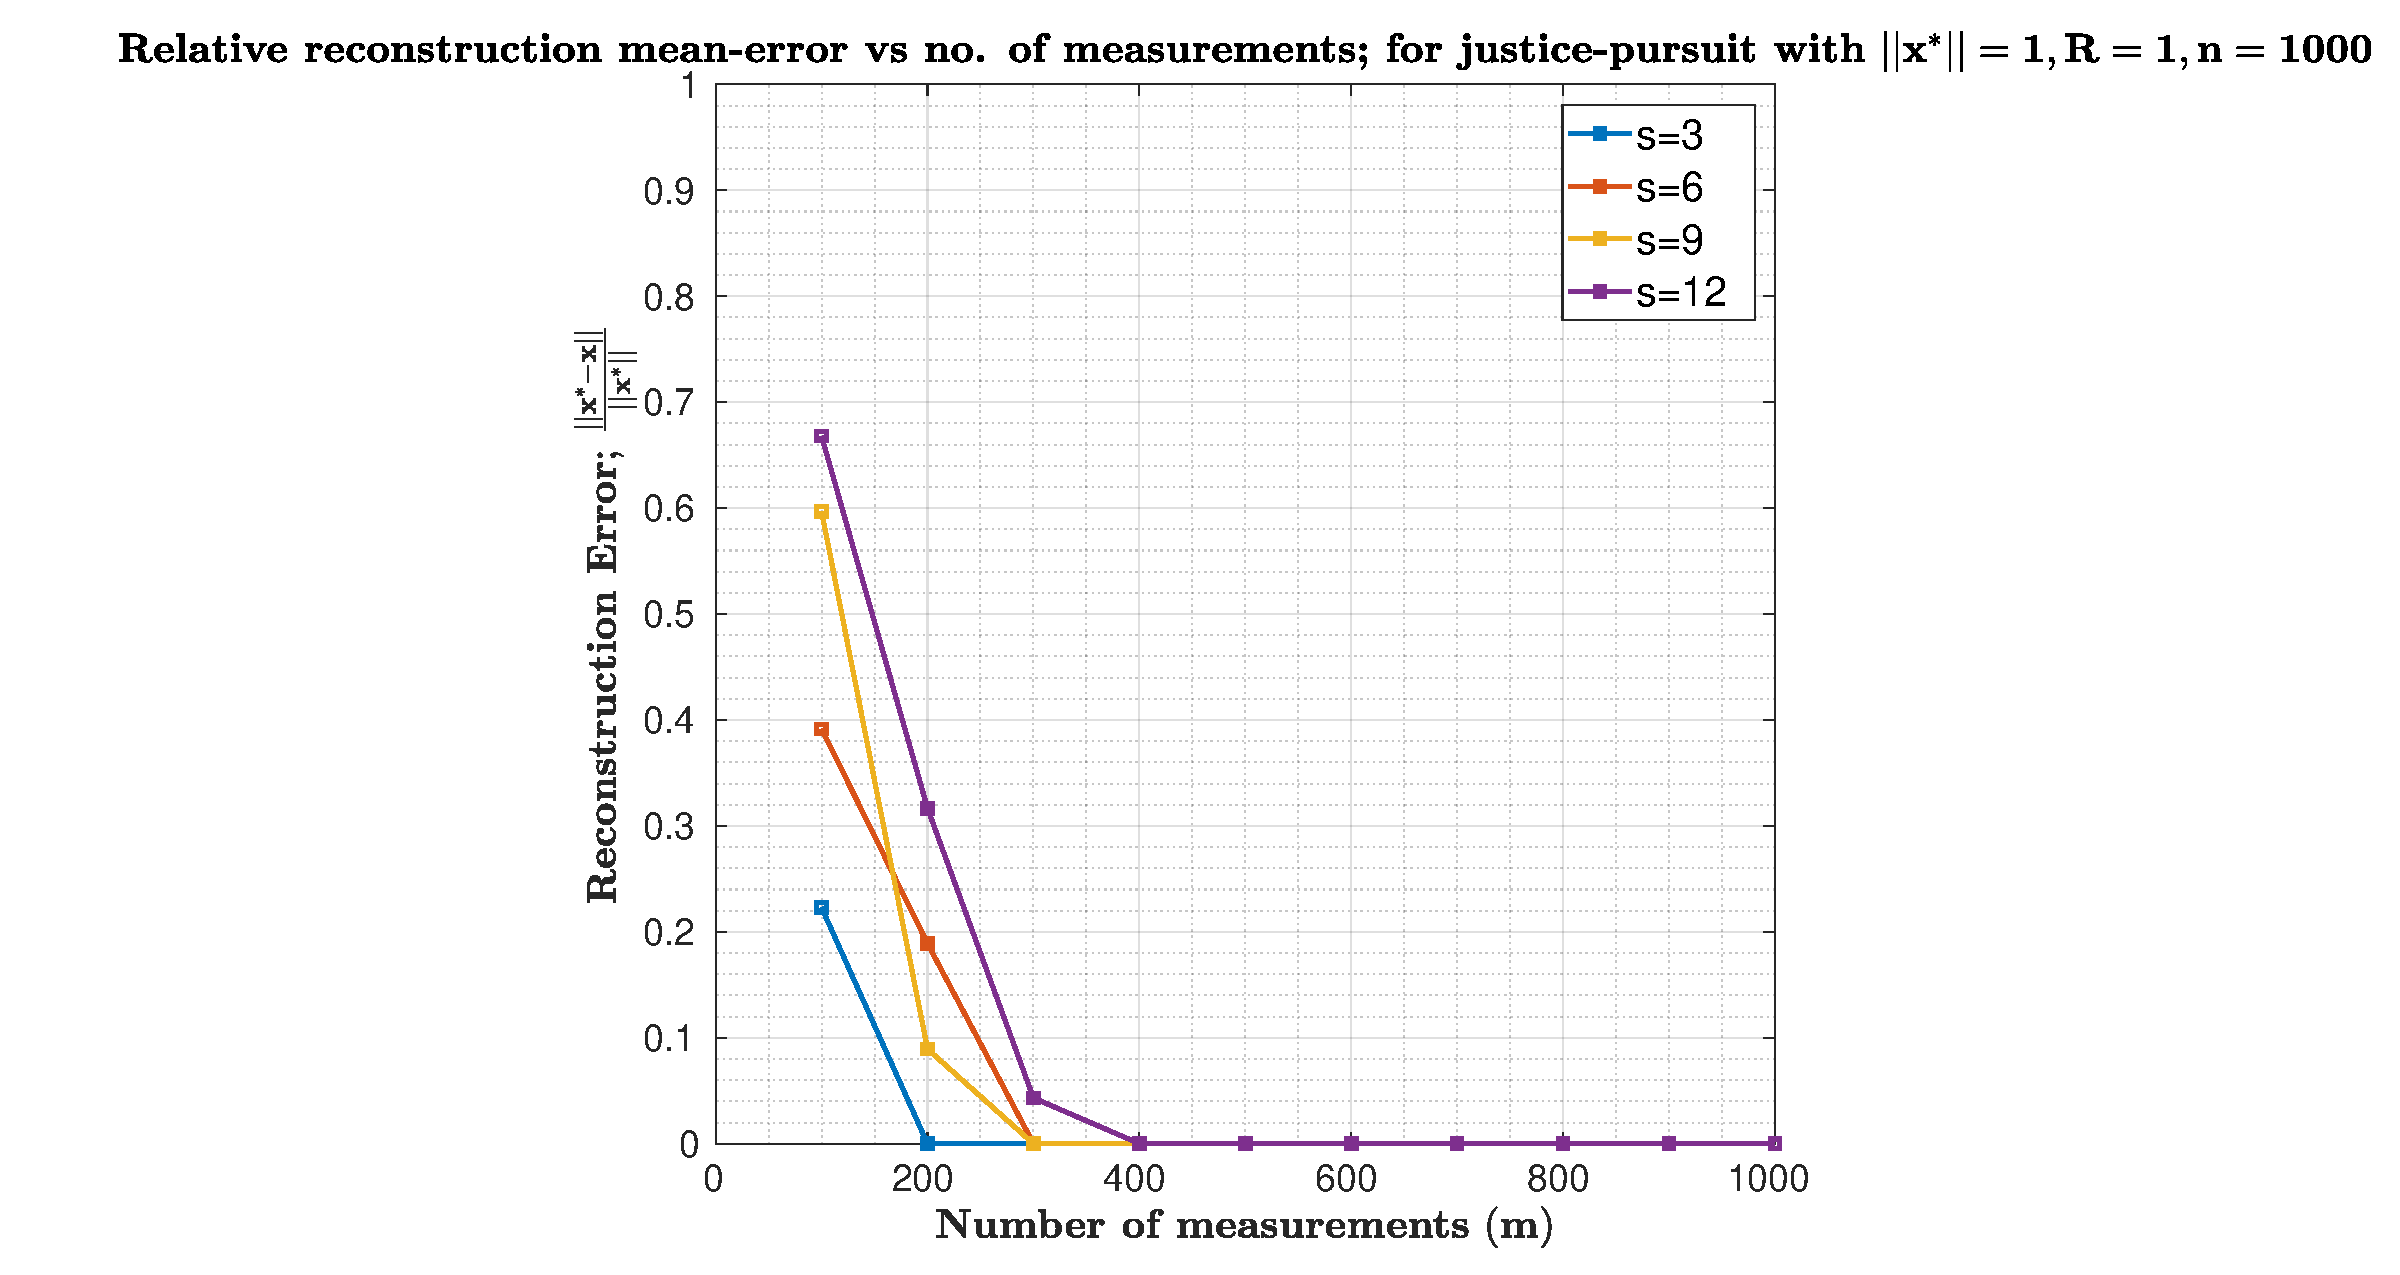
\includegraphics[width=\linewidth]{./fig/plot-1-1_sparse.pdf}
	\end{center}
	\caption{}
	\label{fig:plot-2-1}
\end{figure}


\begin{figure}[h]
	\begin{center}
		%\vspace{-0em}
		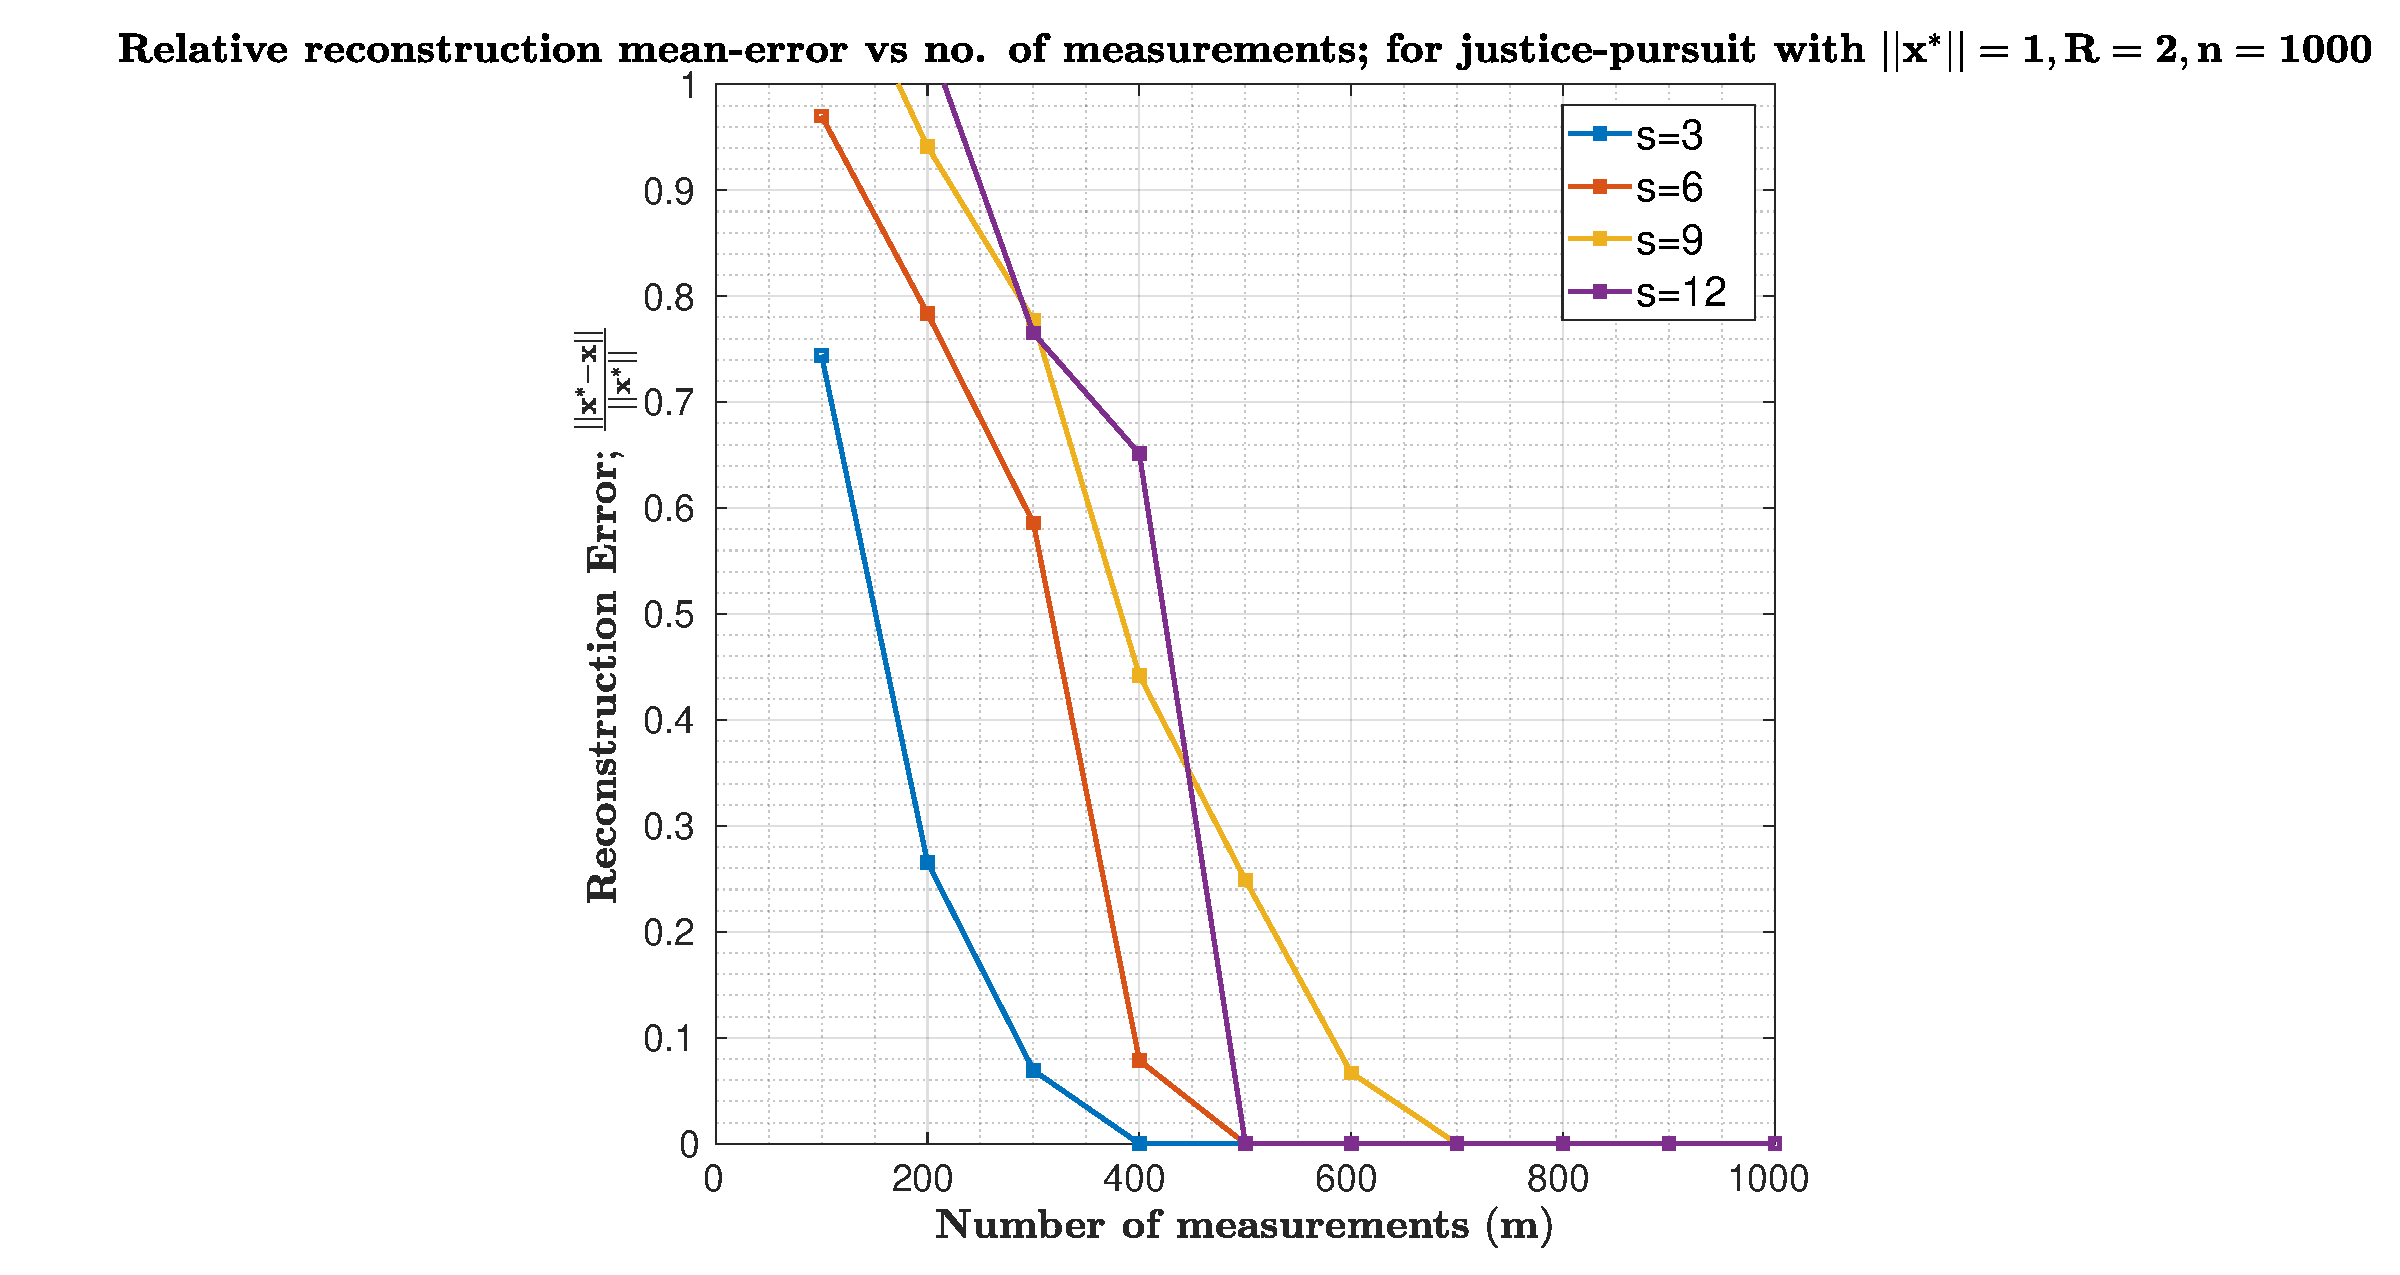
\includegraphics[width=\linewidth]{./fig/plot-1-2_sparse.pdf}
	\end{center}
	\caption{}
	\label{fig:plot-2-2}
\end{figure}


\begin{figure}[h]
	\begin{center}
		%\vspace{-0em}
		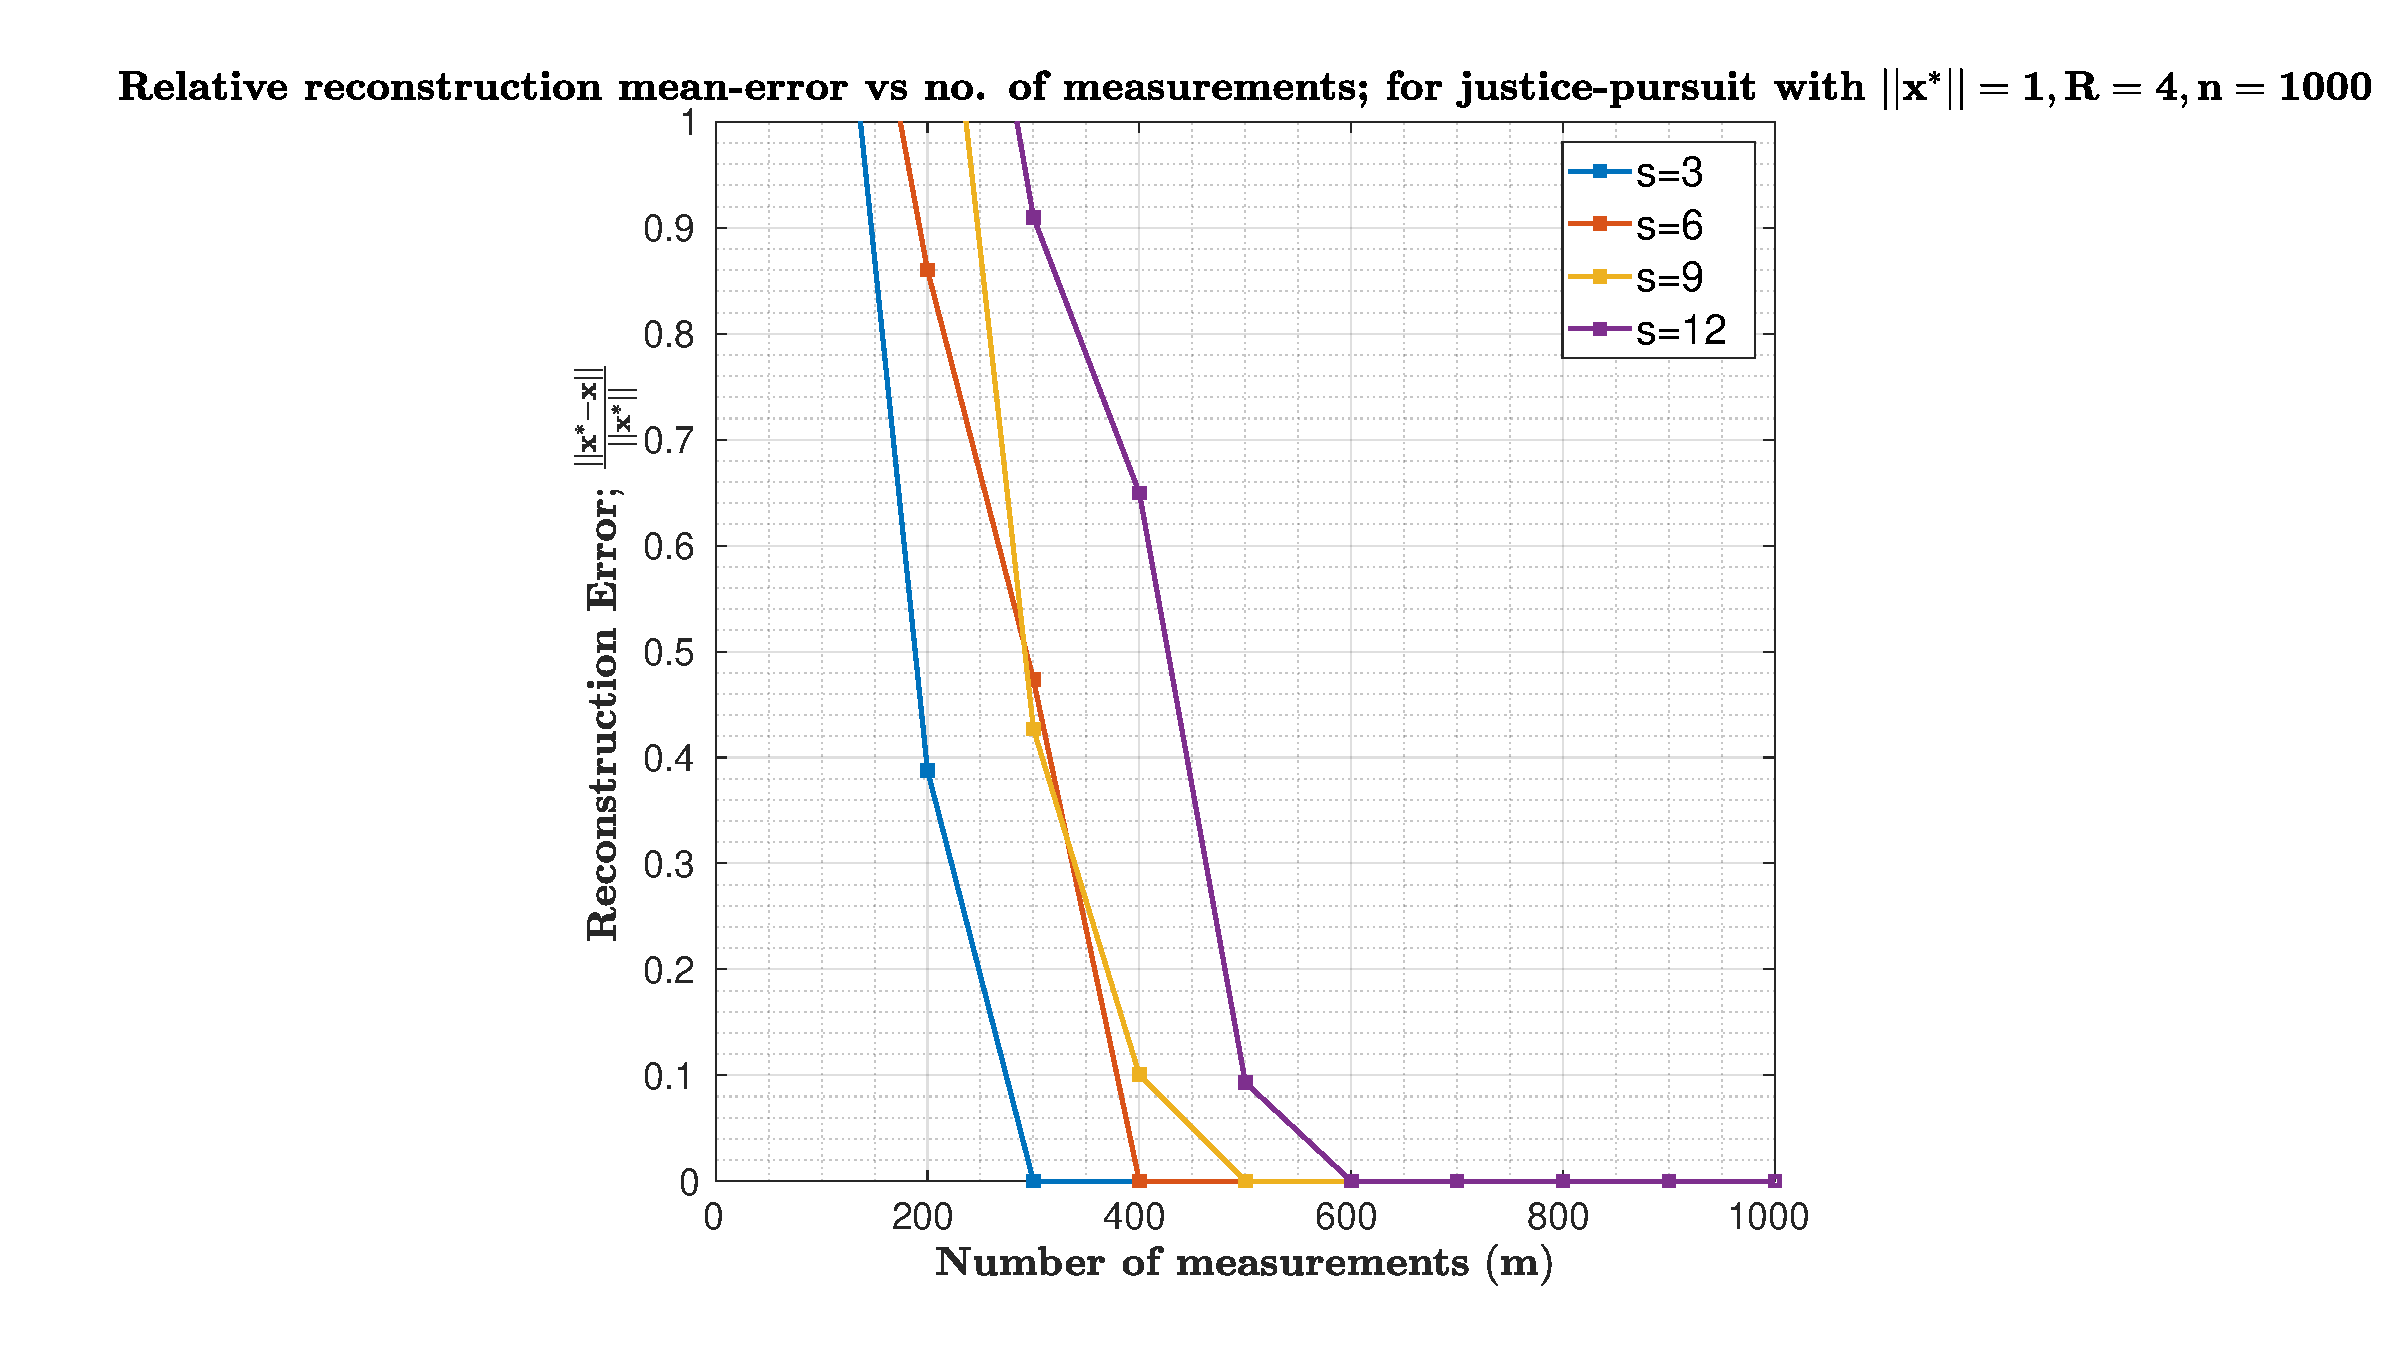
\includegraphics[width=\linewidth]{./fig/plot-1-3_sparse.pdf}
	\end{center}
	\caption{}
	\label{fig:plot-2-3}
\end{figure}